\section{Results}
In this section, we consider the function represent the graph on GUI. As you known in specifications, based on the number of vertices, program automatically pinpoint the vertex's exactly locality.
\\[0.5cm]
Sure, distance between states depend on the radius of circle. As example, with radius is 10 and the graphs are displayed following (see Figure \ref{fig:Figure_1}).
\begin{figure}[h!]
\centering
\subfloat[Graph with 4 vertices]{\label{fig:fig1a}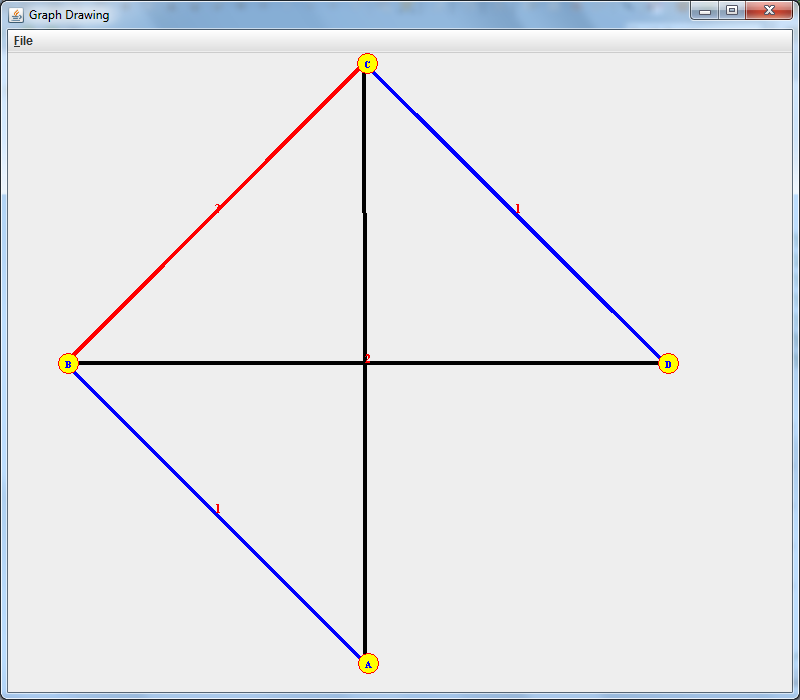
\includegraphics[width=0.3\textwidth]{./images/graph_1}}~~
\subfloat[Graph with 10 vertices]{\label{fig:fig1b}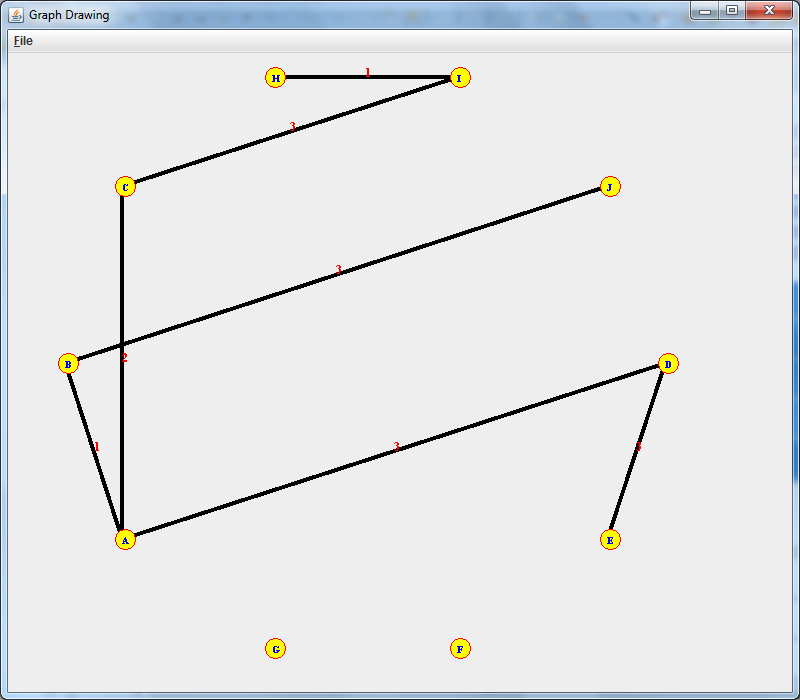
\includegraphics[width=0.3\textwidth]{./images/graph_2}}~~
\subfloat[Graph with 16 vertices]{\label{fig:fig1c}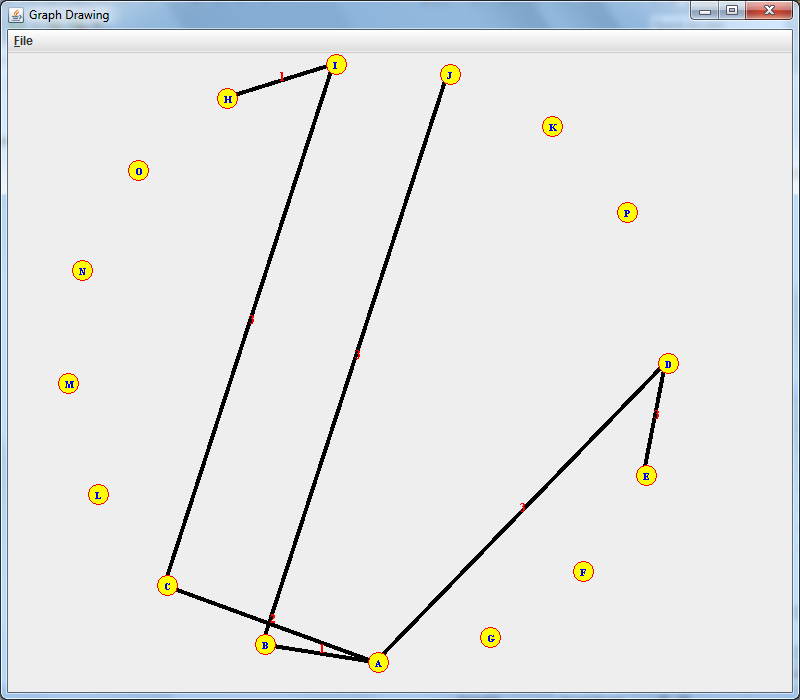
\includegraphics[width=0.3\textwidth]{./images/graph_3}}
\caption{The graph represented on GUI}
\label{fig:Figure_1}
\end{figure}\\
For the graph with 4 vertices, the angular distance between states are 90 degree. Similar, the graph with 10 states, the distance between it is 360 degrees divide by 10, and so on.
\\
The BFS algorithm executes on the graph, when it run on vertex, it make corresponding changes to a action. Besides, the colors of edge also change to form a BFS tree (see Figure \ref{fig:Figure_2}).\\
\begin{figure}[h!]
\centering
\subfloat{\label{fig:fig2a}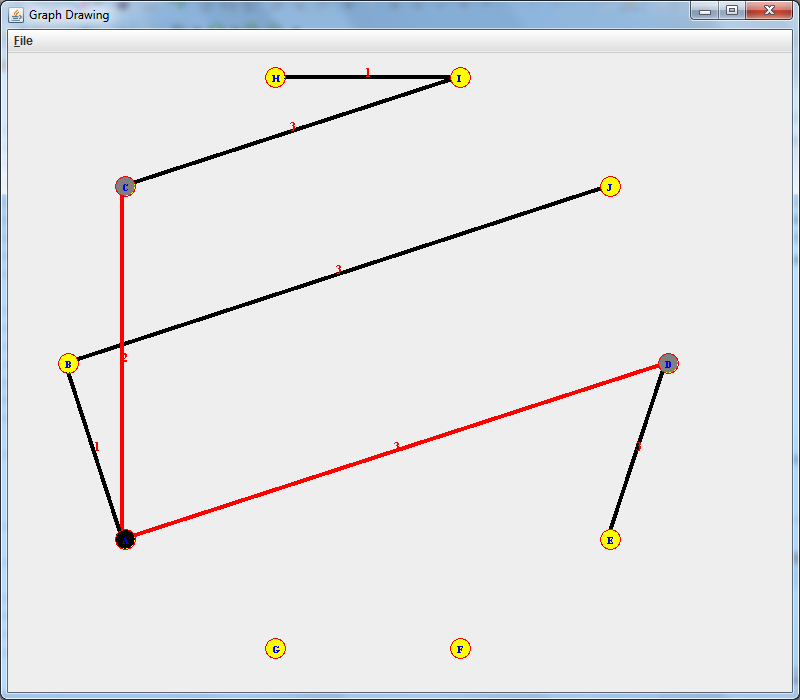
\includegraphics[width=0.35\textwidth]{./images/BFS_1}}~~
\subfloat{\label{fig:fig2b}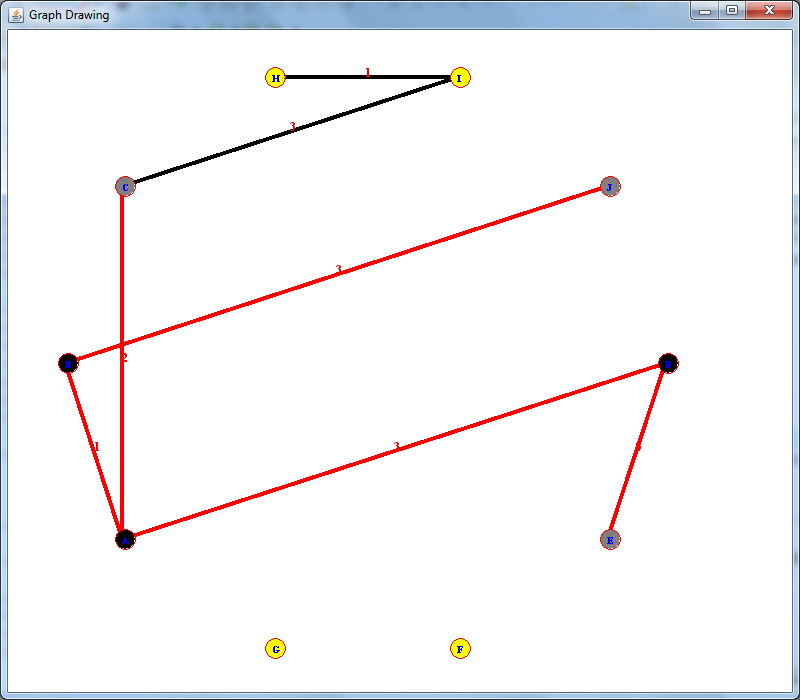
\includegraphics[width=0.35\textwidth]{./images/BFS_2}}
\caption{The BFS algorithm run on graph}
\label{fig:Figure_2}
\end{figure}\\
When the BFS algorithm enqueue a vertex, its color change from yellow to gray. When dequeue it, its color change from gray to black. And, the edge connect by dequeue and enqueue vertex is change from black to red.
\\
The edge coloring algorithm indicate the number of colors to color all edge of graph. After that, it colored the edge such that the graph is valid (Figure \ref{fig:Figure_3}).\\
\begin{figure}[h!]
\centering
\subfloat{\label{fig:fig3a}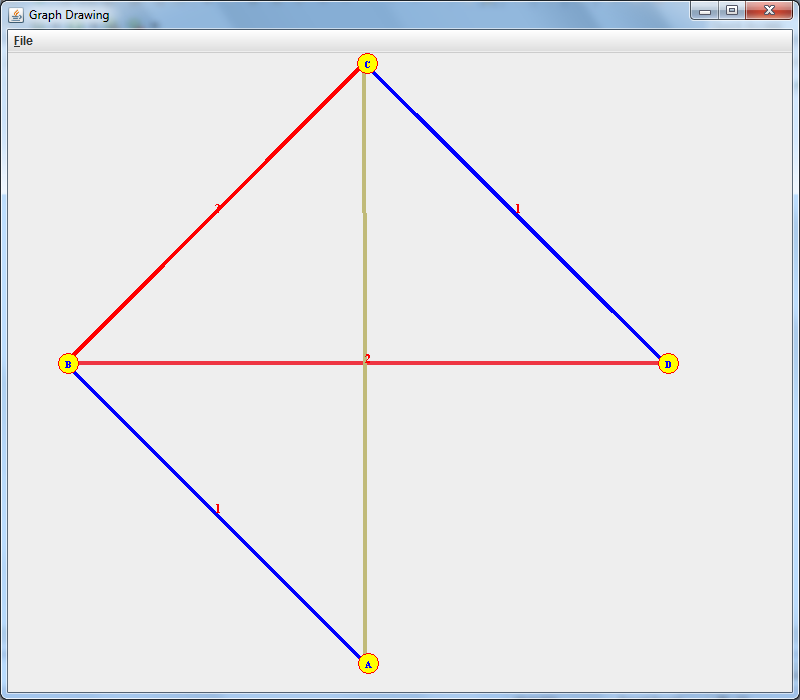
\includegraphics[width=0.35\textwidth]{./images/edge_coloring_1}}~~
\subfloat{\label{fig:fig3b}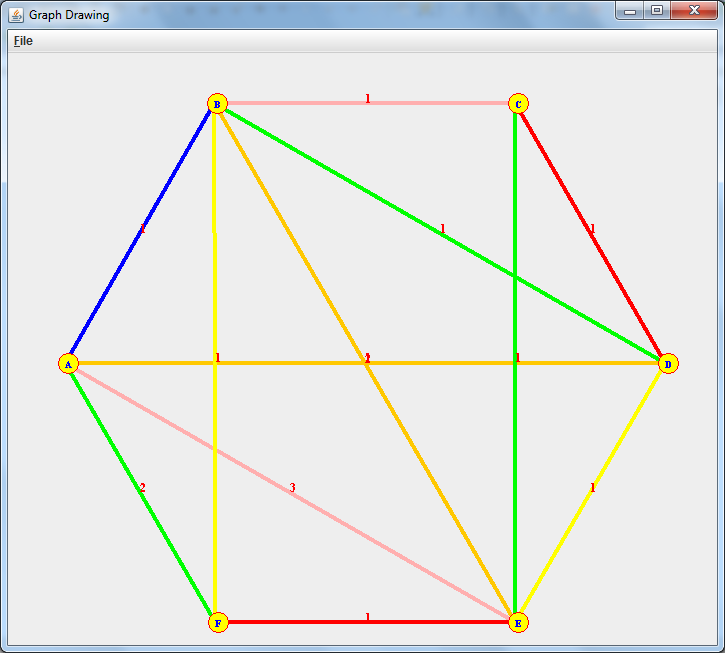
\includegraphics[width=0.35\textwidth]{./images/edge_coloring_2}}
\caption{The graph was colored after execute the edge coloring algorithm}
\label{fig:Figure_3}
\end{figure}\\\\
The edge have black color when it does not colored. We use the colors different black to colored the edge of graph. For every run, the algorithm colored a edge what does not colored. The end, we will have all edge colored. And the number of colors satisfy the Vizing's theorem.
\section{Conclusion}
The application fully the work requirements. Some features are tested in console not in the GUI. The future work would mainly focus on the following functions:
\begin{itemize}
\item Change the way to put the parameters (on GUI).
\item Optimize the code.
\item Integrate more graph algorithm in project.
\end{itemize}